%%%%%%%%%%%%%%%%%%%%%%%%%%%%%%%%%%%%%%%%%%%%%%%%%%%%%%%%%%%%%%%%%%%%%%%%%%%%%%%%
\section*{\centering Part I. Informe Tècnic}
%%%%%%%%%%%%%%%%%%%%%%%%%%%%%%%%%%%%%%%%%%%%%%%%%%%%%%%%%%%%%%%%%%%%%%%%%%%%%%%%

\section{Introducció i Objectius}

Un trie és una estructura de dades en forma d'arbre que utilitza l'indexatge de paraules per organitzar informació. Originalment, els tries van ser pensats per recollir una serie de strings dintre d'un alfabet fixat, però a la computació moderna són àmpliament utilitzades per eines de predicció i cerca a diversos tipus de dades. L'objectiu d'aquest treball és comprendre el funcionament d'aquestes estructures, implementant diferents optimitzacions de les mateixes i avaluant-les experimentalment. 

\section{Antecedents}

L'estructura de dades trie (també coneguda com a arbre de prefixos) és un arbre ordenat utilitzat per representar una sèrie de paraules (strings) sobre un alfabet finit. Permet que els prefixos comuns facin servir els mateixos nodes, i emmagatzema només els caràcters que difereixen. 
Cada node en una trie està associat a un caràcter de l'alfabet, menys el node arrel que és un node buit, i el nombre màxim de fills que pot tenir un determinat node és igual al nombre de caràcters existents en l'alfabet. Pel propòsit d'aquest treball, es farà servir el diccionari ASCII com a referència, de manera que tots els fills quedaran ordenats alfabeticament seguint aquest estandard. El final d'una paraula quedarà representat per un valor associat al node, on s'indicarà l'index d'aquesta paraula dintre del conjunt del text que es faci servir com a dataset. És important recalcar que, per tal que una paraula aparegui al diccionari constituit per un trie, no cal que sigui un node fulla, ja que es pot fer una indexació de qualsevol node intermig que formi part d'una altra paraula més llarga. 

\begin{figure}[H]
    \centering
    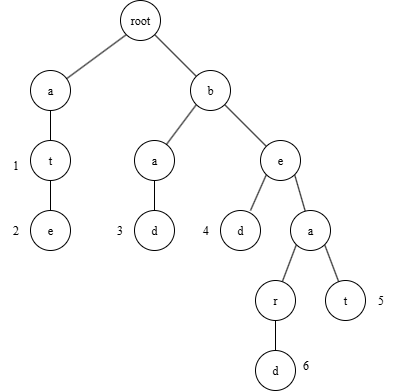
\includegraphics[width=0.6\textwidth]{figures/trie_example.png}
    \caption{Exemple d'un trie que conté les paraules "at", "ate", "bad", "bed", "beard" i "beat".}
    \label{fig:trie_example}
\end{figure}
Tot i que, en general, les tries són estructures eficients per operacions de cerca de paraules o prefixos, aquesta eficiencia normalment significa una penalització en l'ús de memòria. A una implementació bàsica d'un trie, cada node existent tindrà una quantitat de fills igual a la quantitat de caràcters existents en l'alfabet amb el que estem treballant. Això vol dir que en el nostre cas, per exemple, cada node té 128 nodes fills. Notem que a la Figura 1, per simplificació, omitim els fills conformats per nodes buits. 
Per tant, la complexitat espacial d'un trie d'aquest tipus serà de l'ordre de $ O(NM) $, on $N$ representa el nombre de paraules i $M$ la mida màxima d'una paraula. 
 
L'eficiència en termes de memòria ha estat el motor pel desenvolupament de diverses variants de les tries tradicionals. En aquest treball discutirem dues de les principals alternatives: els Ternary Search Trees (TST) i els Radix Trees. 
\subsection{Ternary Search Trees}
Un Ternary Search Tree (o arbre ternari de cerca) és un tipus de trie que busca aprofitar els avantatges espacials dels Binary Search Trees, reduint el numero de fills possibles per un node qualsevol. 
El seu funcionament és simple: cada node tindrà 3 possibles fills. El fill esquerre (\textit{left child}), el fill dret (\textit{right child}) i el fill central (\textit{middle child}). El valor del fill esquerre haurà de ser un valor menor al del node pare, el del fill dret haura de ser major, y el fill central serà un punter al valor del següent símbol de la string a qui pertany el node central.
Notem que el rendiment d'aquesta estructura depen directament de la profunditat de l'arbre.  


\section{Disseny i Implementació}

En aquest apartat cal descriure amb detall les decisions de disseny i les implementacions realitzades. Cal explicar quines estructures s’han utilitzat, com s’han representat internament i quines operacions s’han implementat (com ara inserció, cerca, autocompletat, etc.), tot destacant com s’ha garantit l’eficiència de cadascuna. També és convenient discutir les possibles alternatives que s’han considerat durant el desenvolupament, així com justificar les opcions escollides. Finalment, s’hauria d’incloure una comparació qualitativa entre les diferents implementacions desenvolupades, tot valorant-ne avantatges, limitacions i aplicabilitat en funció de l’escenari o conjunt de dades.

\section{Avaluació Experimental}

Aquí cal presentar l’anàlisi empírica del rendiment de les estructures implementades. Es poden descriure els conjunts de dades emprats, les proves realitzades, les mètriques recollides (temps d’execució, memòria, nodes visitats, profunditat mitjana, etc.) i mostrar els resultats obtinguts de manera gràfica o tabulada. Finalment, s’hauria de fer una interpretació crítica dels resultats, contrastant-los amb les expectatives teòriques.

\section{Conclusions}

En aquesta secció s’han de resumir els principals resultats i aportacions del projecte. Es pot fer una valoració del rendiment assolit, de les dificultats trobades i del coneixement adquirit. També és pertinent incloure possibles extensions, millores o línies futures de treball si el projecte es volgués ampliar. Aquesta secció hauria de tancar el document de forma clara i reflexiva.
